\documentclass[lang=cn,a4paper]{elegantpaper}

\title{数学建模}
\author{作者:陶理 \\ 中三(2)班  28号}
\institute{上海市实验学校}
\date{\zhtoday}

\usepackage{url,appendix,graphicx,float,multicol}
\begin{document}

    \maketitle

    \section{第一题}
    \subsection{问题分析}
    \subsubsection*{分析方式}
    编程:python语言

    所需第三方库:numpy,matplotlib
    
    将题目所给的x、y数据转化为python中的list数据类型(即数组),通过plotfit函数进行多项式拟合。
    \subsubsection*{判断耦合程度}
    思路来源:方差和标准差
    $$
    s^2=\frac{1}{n}\sum_{i=1}^n (a_i-\bar{a})^2,s=\sqrt{\frac{1}{n}\sum_{i=1}^n (a_i-\bar{a})^2}~~~~~~~~~~~~(\bar{a}=\frac{1}{n}\sum_{i=1}^n a_i)
    $$

    记原本的数值是$x_i$对应$y_i(1\leqslant x\leqslant n,x\in \mathbb{Z}^+)$

    记拟合函数为$f(x)$,使用拟合函数预测的数值为$p_i=f(a_i)~~(1\leqslant x\leqslant n,x\in \mathbb{Z}^+)$
    
    通过$p_i$和$b_i$之间的误差可以判断拟合函数f(x)和原曲线的耦合程度,误差越小说明耦合程度越好。
    $$
    \Delta^2=\frac{1}{n}\sum_{i=1}^n (p_i-b_i)^2, \Delta=\sqrt{\frac{1}{n}\sum_{i=1}^n (p_i-b_i)^2}
    $$
    \subsection{拟合结果}
    三次:$y=3.734x^3-150.8x^2+1251x-2447$
    
    $\Delta_3=6146.0500$
    \begin{figure}[H]
        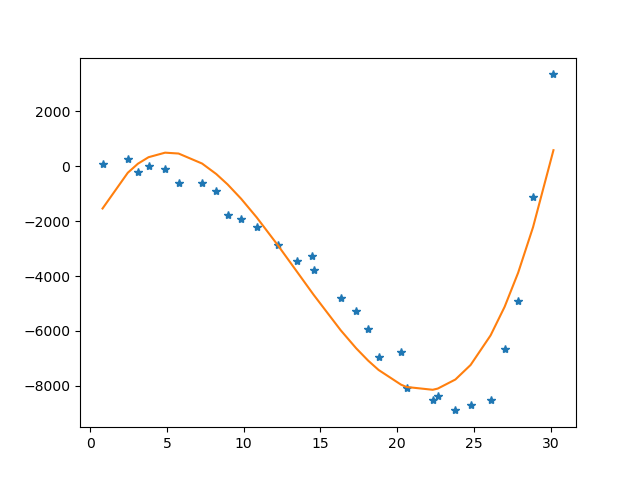
\includegraphics[scale=0.4]{1-3.png}
    \end{figure}
    四次:$y=0.2556x^4-12.13x^3+169.2x^2-1041x+1633$
    \begin{figure}[H]
        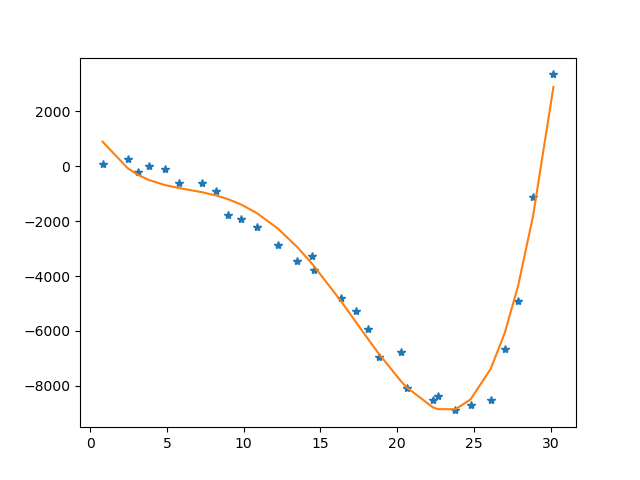
\includegraphics[scale=0.4]{1-4.png}
    \end{figure}
    五次:$y=0.01262x^5-0.7224x^4+15.01x^3-152.9x^2-464.9x-236.6$
    \begin{figure}[H]
        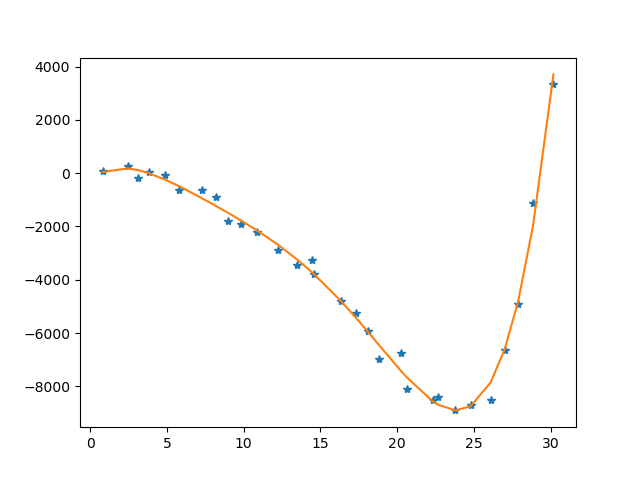
\includegraphics[scale=0.4]{1-5.png}
    \end{figure}
    六次:$y=-5.661\times 10^{-5} x^6+0.01787x^5-0.9075x^4+18.09x^3-177.4x^2+545.3x-309.3$
    \begin{figure}[H]
        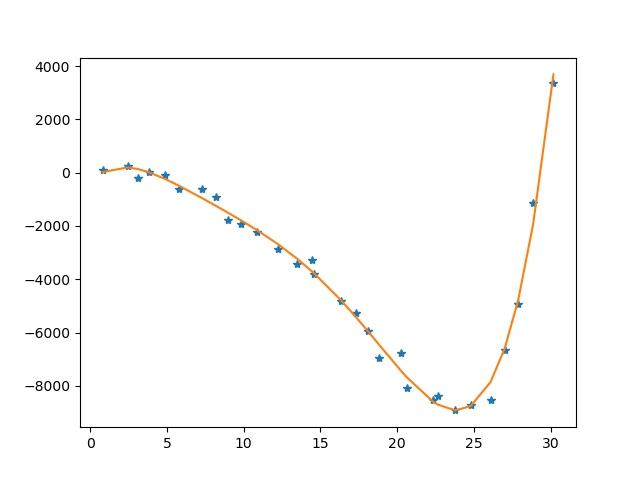
\includegraphics[scale=0.4]{1-6.png}
    \end{figure}
    七次:$y=-5.622\times10^{-5}x^7+0.006036x^6-0.2443x^5+4.778x^4-47.04x^3+198.1x^2-382x+331.3$
    \begin{figure}[H]
        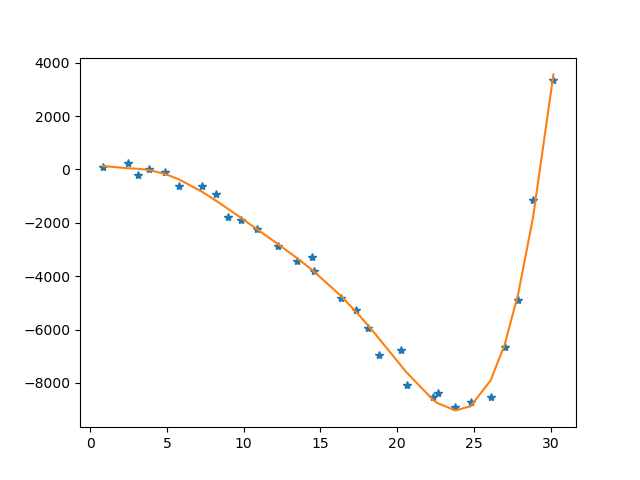
\includegraphics[scale=0.4]{1-7.png}
    \end{figure}
    \clearpage

    \section{第二题}
    \subsection{问题分析}
    \subsubsection*{题目:}
    小旭家现有1千克馄饨/饺子馅,小旭准备自己动手包一些馄饨/饺子,他想知道需要准备多少馄饨/饺子皮。试建立数学模型,讨论对于肉馅或菜肉馅、对于方形的馄饨皮或圆形的饺子皮,1千克馅料分别需要多少面皮可以恰好把所有馅料做成馄饨/饺子?
    \subsubsection*{条件:}
    \begin{itemize}
        \item 有1kg的馄饨/饺子馅
        \item 馄饨皮是方的,饺子皮是圆的
        \item 馅有两种选择:肉馅或菜肉馅
    \end{itemize}
    \subsubsection*{分析:}
    问1kg馅料分别需要多少面皮可以恰好把所有馅料做成馄饨/饺子,其实可以等效看作1kg的馅料可以包多少馄饨/饺子。而这个问题可以最终看作一个饺子能包多少质量的馅料,即一张面皮对应的馅料的质量。

    根据化简后问题“一张面皮对应的馅料的质量”以及物理公式$m=\rho V$,需要知道馅料的密度以及一张面皮中能放多少体积的馅料。而一张面皮中能放多少体积的馅料取决于面皮的大小,所以需要设定面皮的边长或者直径(或半径)。
    \subsection{建立模型}
    将馅料看作一个椭球体(如下图所示)。
    \begin{figure}[H]
        \centering
        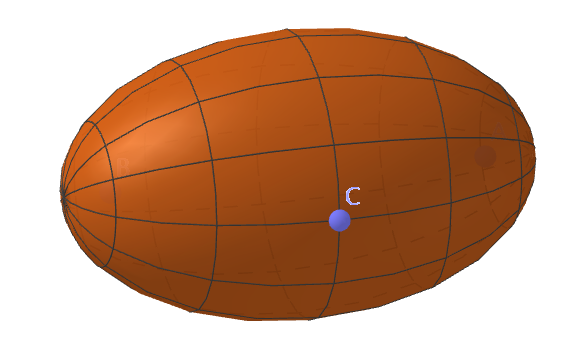
\includegraphics[scale=0.2]{ellipsoids.png}
    \end{figure}
    将馄饨皮近似看成以a为边长的正方形(如图所示)
    \begin{figure}[H]
        \centering
        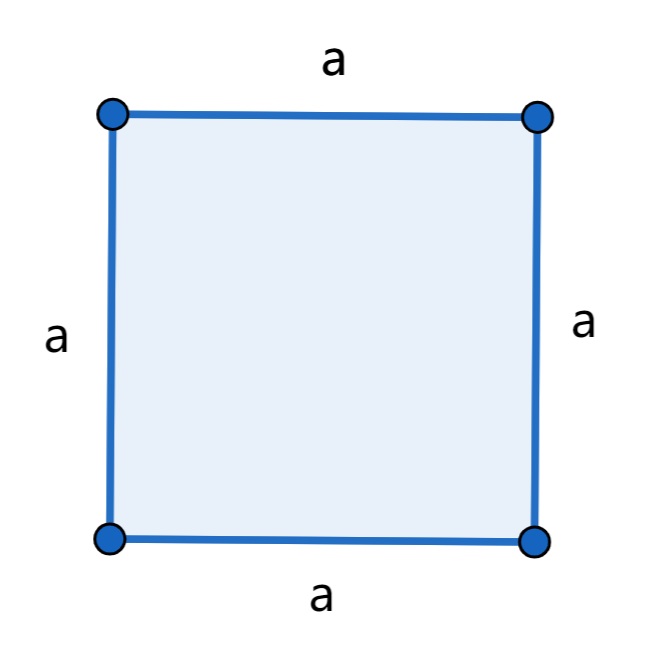
\includegraphics[scale=0.5]{square.png}
    \end{figure}
    将饺子皮近似看成以a为半径的圆
    \begin{figure}[H]
        \centering
        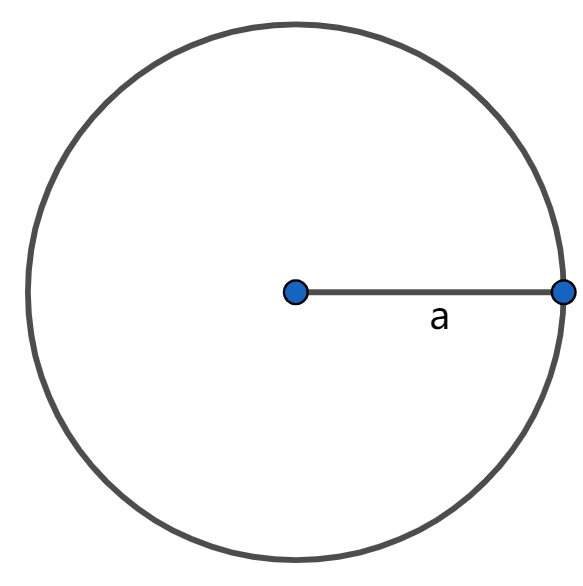
\includegraphics[scale=0.4]{circle.png}
    \end{figure}
\end{document}
